\section{User Interface}
\label{sec:gui}
The implementation of the user interface is described in this section. Since the GUI has been developed iteratively, each subsection describes the progress gained in the corresponding sprint. In addition, section \ref{sec:GuiTest} discusses the method used for testing the interface.
\subsection{Second Sprint}

In this sprint, the first iteration of the user interface was developed, first a character user interface as described in the  \hyperref[sec:CUI]{\textit{Character User Interface}} section and following a graphical user interface as described in the \hyperref[sec:GUIS1]{\textit{Graphical User Interface}} section. The issues found while developing the interface are discussed in the \hyperref[sec:LimS1]{\textit{Limitations}} section.
\subsubsection{Character User Interface}
\label{sec:CUI}
The first iteration for the user interface was a simple CUI (Character User Interface) which directly shows the data which is gathered from the sensors and sent through the wireless connection. Because of the fact that Matlab, the chosen framework for user interface, contains an inherent CUI, there was no need to create a custom CUI. Because of this, the implementation of the CUI consisted of creating a receiver for the sensor data and transforming this data in a readable format as can be seen in figure \ref{fig:CUIV1}. 

\begin{figure}[H]
	\centering
	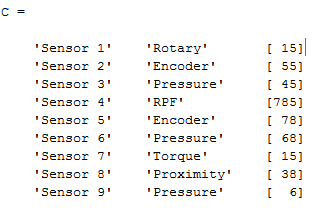
\includegraphics[width=.75\textwidth]{images/CUI}
	\caption{A sample of the CUI} 
	\label{fig:CUIV1}
\end{figure} 

\subsubsection{Graphical User Interface}
\label{sec:GUIS1}
The GUI (Graphical User Interface) was made using Matlab graphical elements. Initially, the GUI contained two graphs and two tables, one table which shows all the sensors and one which shows only a selection of important sensors as can be seen in figure \ref{fig:GUIV1}.
The table of important sensors is intended to show more details about the selected sensors while the table of all sensors is intended to give a quick overview of all sensors. The GUI contains two graphs as well which both plot the current as well as previous values of the selected sensor. When a sensor is selected in the table of all sensors, all properties of this sensor will be shown and can be edited. A property of special note is the 'SI-Prefix': in the table of important sensors, the SI-Prefix of a sensor can be changed, and the value will be scaled accordingly. 

\subsubsection{Limitations}
\label{sec:LimS1}
The Matlab UITable class, which was used to show the data, has the disadvantage that the entire table has to be redrawn if something changes, even if only one cell changes. Since redrawing an entire table takes about $0.05$ seconds, 
doing this every update is not a possibility with an update rate of 50 Hz. Of course, having such an high update rate would make the table completely unreadable, since the data changes before one has even time to read it. In addition, in order to remove unnecessary redrawing, the static and dynamic parts of the tables are split where possible. Another problem introduced by the high refresh rate is that callback functions which are triggered by editing table cells do not function correctly. Because of the high update rate, the table is redrawn before the callback function has finished which gives unintended results. This problem has been solved by moving all cells with an edit callback to a table with a low refresh rate. 

\begin{figure}[H]
	\centering
	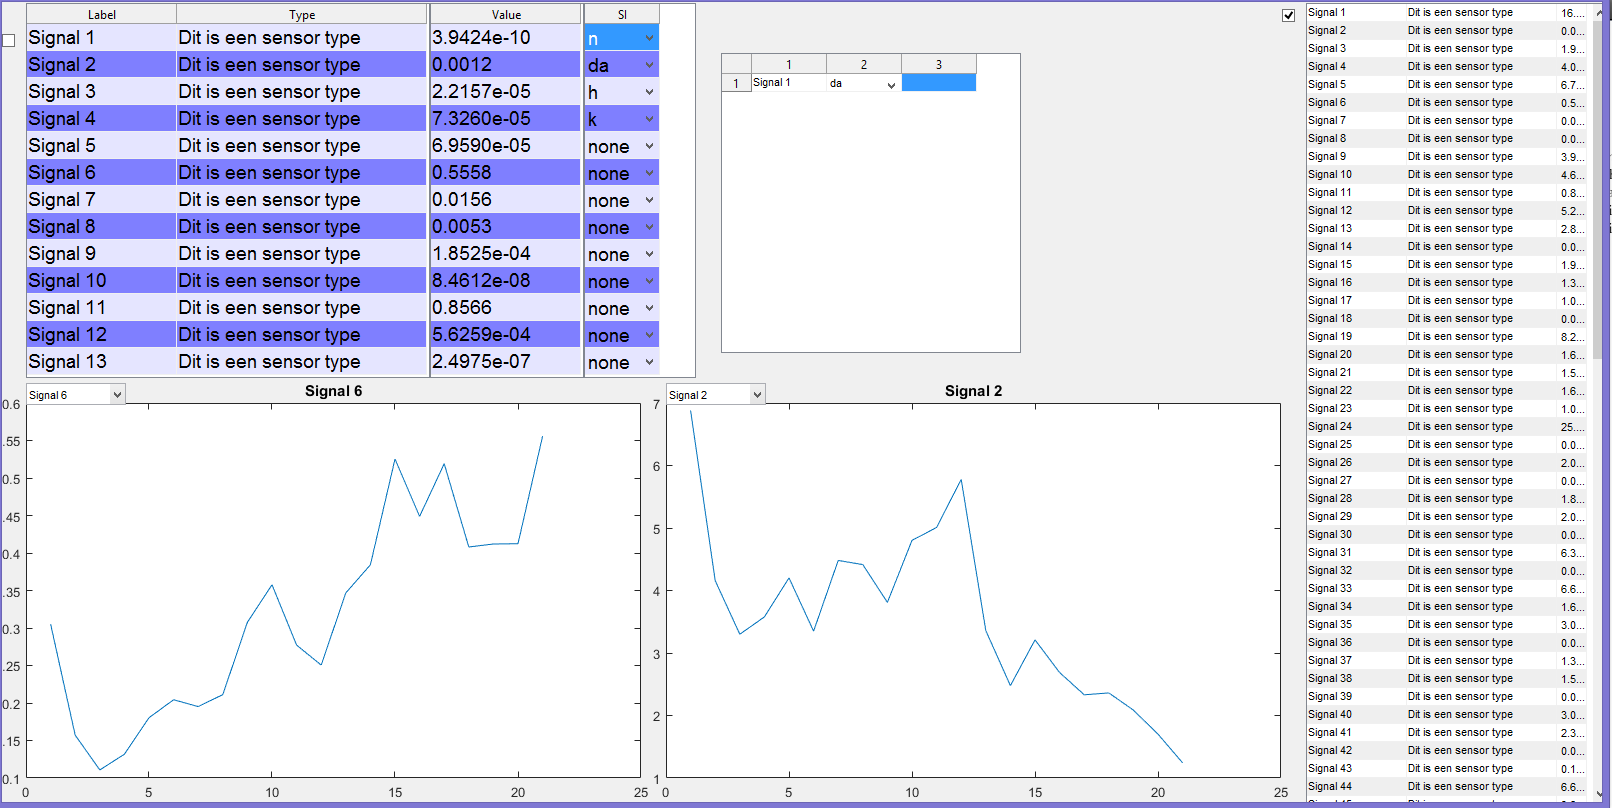
\includegraphics[width=.75\textwidth]{images/GUIV1}
	\caption{A sample of the GUI at the end of the second sprint} 
	\label{fig:GUIV1}
\end{figure} 

\subsection{Third Sprint}
In this sprint the graphical user interface was refined. The implementation of more visualisation functionality is discussed in the \hyperref[sec:VisS3]{\textit{Visualisation}} section. The implementation of additional control tools in the interface is discussed in the \hyperref[sec:ConS3]{\textit{Control}} section. The limitations found in the implementation of this sprint is found in the \hyperref[sec:LimS3]{\textit{Limitations}} section .
\subsubsection{Visualisation}
\label{sec:VisS3}
For each sensor has an minimum and maximum safe value. When a value is not between these values, the sensor is marked red so it is immediately clear that there is something wrong. When a sensor is selected, one can see its minimum and maximum values. It is also possible to add multiple sensors to a graph in order to easily compare their values. It should be noted that the graphed data is not normalised, so visualising sensors with widely different data ranges is not advised.  

\subsubsection{Control}
\label{sec:ConS3}
The dimensions of all visual elements are static in order to have better control over the visual representation. To accommodate people with small screens, it is possible to toggle between two predefined sizes. These are defined in a separate configuration file which also contains other data which should be editable like the update rate of separate components and whether the sensor data is generated local or received over network. In the sensor property window, it is possible to toggle whether a sensor is in the table of important sensors. Additionally, the values of a sensor can be given a transformation as well by entering the corresponding formula in the formula field in the sensor property window as is shown in figure \ref{fig:GUIV2} . 


\subsubsection{Limitations}
\label{sec:LimS3}
Showing which sensors have exceeded their minimum or maximum values is one of the most important features of the Monitoring System according to the members of the Project MARCH team, since this means that something has gone seriously wrong with the exoskeleton. Therefore each update, the sensor values are checked if they do not exceed the minimum or maximum values. If a value lies outside this range, the table of sensors is redrawn immediately with the offending sensor marked red. While testing with data which frequently exceeds the minimum/maximum values, it turned out that this heavily impaired the performance as the table of sensors gets rendered a lot more frequently compared to usual use. However, since receiving outliers in the sensor data is supposed to be exceptional and an indicator that something is broken in the exoskeleton, performance is subsidiary to showing that there is something wrong.


\begin{figure}[H]
	\centering
	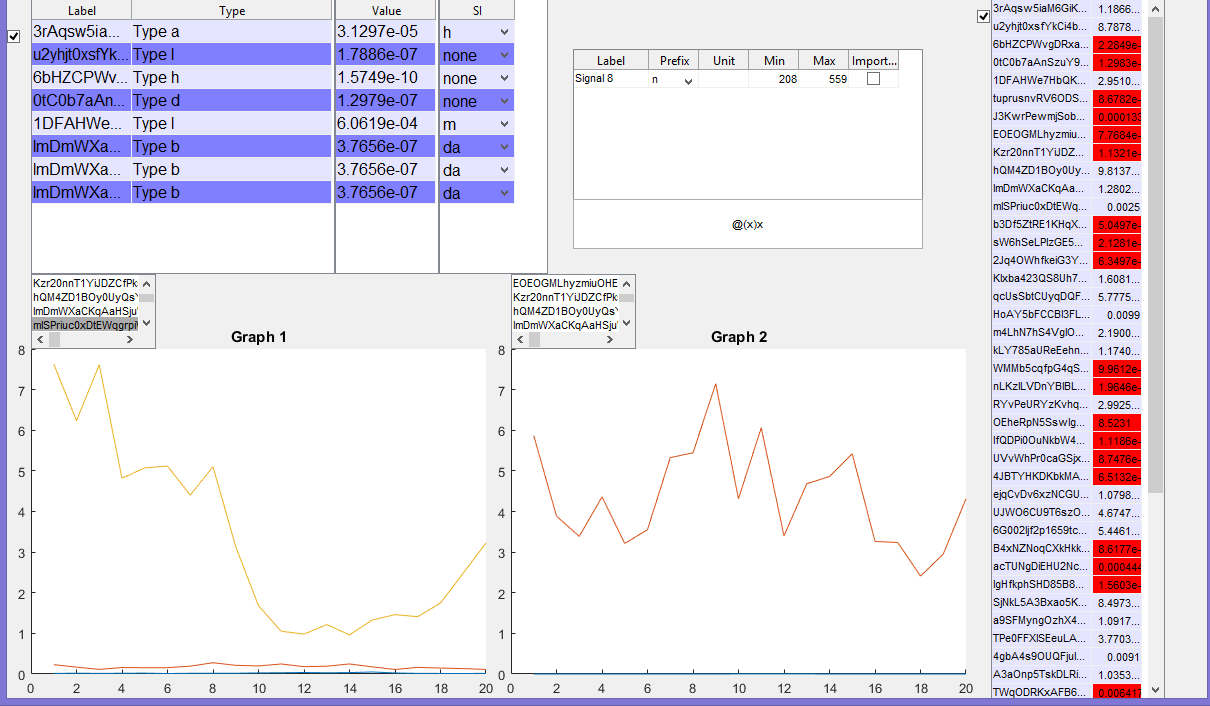
\includegraphics[width=.75\textwidth]{images/GUIV2}
	\caption{A sample of the GUI at the end of the third sprint} 
	\label{fig:GUIV2}
\end{figure} 

\subsection{Fourth Sprint}
In this sprint the graphical user interface was finished. The performance issues and the solution for them is discussed in the \hyperref[sec:PerfS4]{\textit{Performance}} section . The last additions to the interface are discussed in the \hyperref[sec:GUIS4]{\textit{Interface}} section. 

\subsubsection{Performance}
\label{sec:PerfS4}
When testing for performance, the Matlab profiler showed that the function used to plot the graphs took a lot of time. It turned out that the functions used to plot and clear the graphs have more functionality than just plotting a line and therefore have 	unnecessary overhead. In order to solve this problem, instead of using a plot function, a line object is created for each graph. If the line object is updated, only the line is redrawn instead of the entire graph. This resulted in a huge performance boost which increased the best case update rate from 20 Hz to 100 Hz.\\

Now that it is possible to have an update rate for the GUI which is higher than the update rate of the data packages, the GUI needs to be able to deal with an empty queue of packets. In earlier iterations of the system, this was done by repeating the latest data in the update function. However, this makes it seem that there is new data when there is none. This has been changed in a wait-loop which waits if there is no packet in the queue and otherwise runs the regular update flow as can be seen in figure \ref{fig:UpdateFlow}. 
\begin{figure}[H]
	\centering
	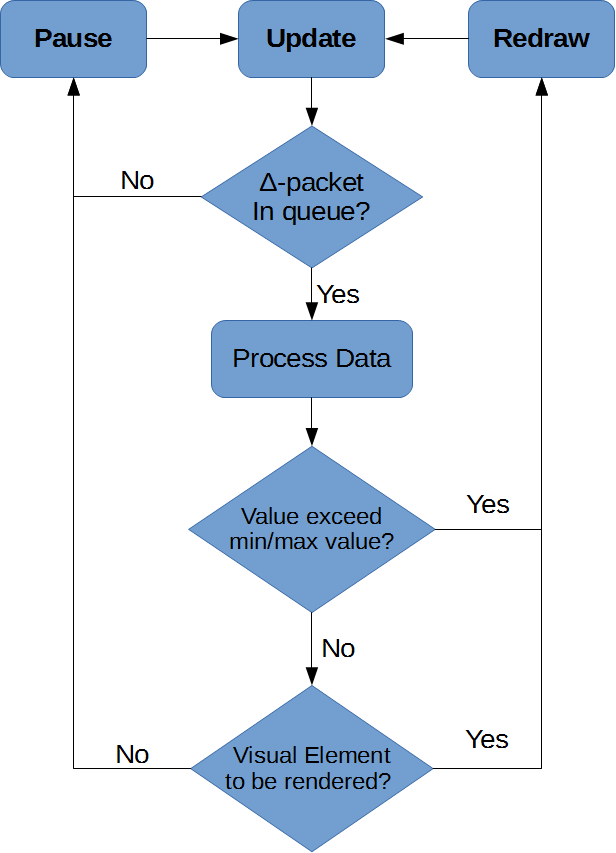
\includegraphics[width=.6\textwidth, height=0.5\textheight]{images/UpdateFlow}
	\caption{Diagram which shows how the update flow is structured} 
	\label{fig:UpdateFlow}
\end{figure} 
\subsubsection{Interface}
\label{sec:GUIS4}
In the previous iterations of the GUI, the used resolution for the GUI was 1600x800. However, quite a number of laptops have a screen resolution of 1900x1080. In order to make optimal use of this, an additional lay-out for 'large' monitors was created. The extra space was utilised to add some more graphs to the GUI, giving the option of showing up to four graphs, each which can be linked to multiple sensors. The graphs were also given legends in order to easily discern which line corresponds with which sensor. 
In order to move control from the console to the GUI, several togglable settings have been compiled in list of checkboxes instead of settings in the configuration file or being hardcoded. This is done to make starting functions like starting updating or recording easier and to temporarily disable performance draining components.
Since rendering at an high frequency makes the information blur over before the user has even the chance to properly interpret the data, the components of the GUI should not be updated every time the data is updated. In order to maximise control for the user of the GUI, the length of the pause as well as the update rate of different components of the GUI can be directly set in the GUI as all can be seen in figure \ref{fig:GUIV3}



\begin{figure}[H]
	\centering
	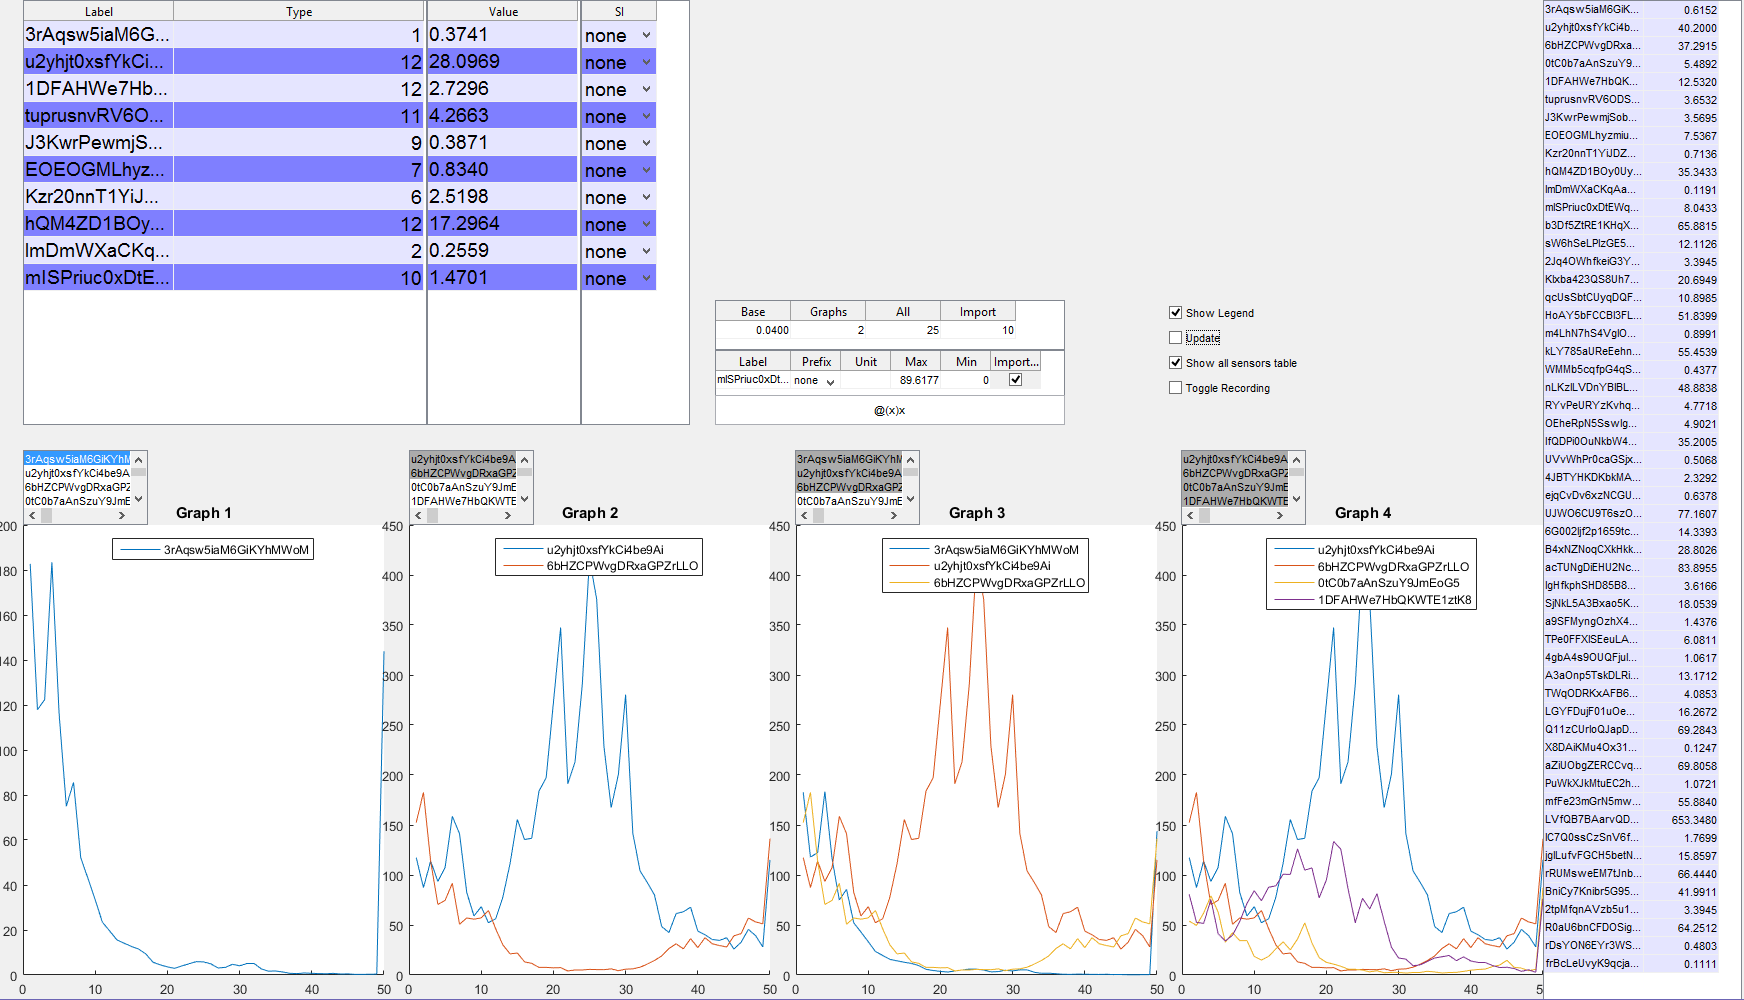
\includegraphics[width=.75\textwidth]{images/GUIV3}
	\caption{A sample of the GUI at the end of the fourth sprint} 
	\label{fig:GUIV3}
\end{figure} 

\subsection{Testing} 
\label{sec:GuiTest}
Testing the GUI was done by exploratory testing because the most important aspect of the GUI that needed to be tested was whether the GUI behaves as the user would expect and if the data is shown correctly. Because of the fact that the Simulink-model was continuously sending predictable test data, it was easily visually deducible whether a certain function works correctly.  In addition, non-functional testing was done with the Matlab profiling tool to test for performance of the several elements in the GUI. 